\chapter{Introduction}
\label{cha:intro}


\section{Motivation}

Deafness is estimated to be the fourth leading disability globally \cite{deafness_4th_disability}. In 2018, the \acrlong{who} reported that 466 million people (over 6.1\% of the world's population) were affected by \acrfull{dhl} \cite{WHO_rising_hearing_loss}. This is estimated to reach 700 million people by 2050 \cite{WHO_deafness_stats}. If accurate, one in ten people will be affected by deafness.\\
This trend would mean that treatments for \acrshort{dhl}, such as cochlear implants and hearing aids, will rise in demand in the coming years. Accessibility features in videos, like closed captions and sign language, will become more critical. Currently, these technologies are powered mainly by processing audio clips and synchronising them in real-time to the correct place within videos. However, this is harder to do in real-time and is made even more difficult by a range of factors. Accent, \gls{speech_disfluency} and background noise can hugely impact the transcription of words being said.\\
A major factor that impacts speech processing is the shape of the moving mouth, even in those without hearing loss~\cite{lip_reading_used_by_everyone}. Incorporating visual components, in addition to audio, provides more precise speech processing results \cite{audio-visual_processing_better}.\\
Utilising visual components could improve speech recognition technology. For noise, being able to select a single talker and focus on their speech could help an individual with hearing loss to understand them. Modern-day speech recognition would become confused within this noisy environment (unless uni-directional microphones were used), possibly trying to listen to many speakers at once. This technology wouldn't just aid those with \acrshort{dhl} but also individuals with auditory processing disorders, such as Autism.\\
Currently, no software supports this functionality and there is little existing software able to overcome the difficulties present within speech.\\
Most people with \acrshort{dhl} live in low- and middle-income countries \cite{WHO_deafness_stats} and therefore have poorer access to medical treatment for their condition. Education within these regions may also be lacking, leading to individuals not learning the necessary skills to understand those around them~\cite{cochlear_implants_low_income, Disability_in_low-income...}. Without treatment, for hearing loss, deafness can become debilitating.\\
Therefore, there is a high, and rising, demand for software able to use visual cues for lip reading. With an increasing proportion of the population suffering from \acrshort{dhl}, treatment and accessibility are becoming far more important. Visual lip reading could be used to improve current speech recognition software, aid those with hearing and auditory processing conditions, and educate people first learning how to read lips.

\section{Machine Learning for Lip Reading}
\begin{figure}
\centering
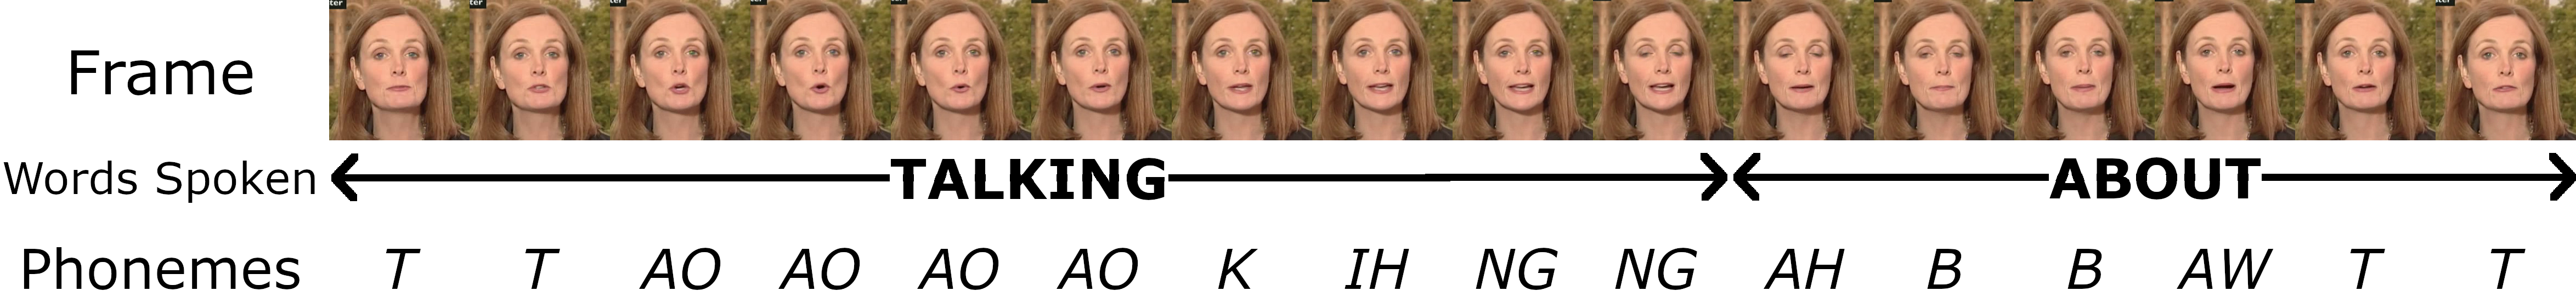
\includegraphics[width=0.9\textwidth]{resources/LRW Example.png}
\caption[A lip reading example from \gls{lrw}.]{A lip reading example from \gls{lrw} \cite{Lip-Reading-In-The-Wild}. This shows the temporal nature of speech, with words spread across frames and being comprised of \gls{phoneme}s. In the example, two words are said: ``TALKING" and ``ABOUT".}
\label{fig:LRW Example}
\end{figure}
\acrfull{ml} is now used for all manner of applications to great success. From stock market prediction to image recognition and even generating artwork, \acrshort{ml} can carry out all manner of complex jobs.\\
Lip reading using \acrshort{ml} is cheap, fast and can be improved over time. \acrshort{ml} models possess the complexity to capture essential nuances within data. Lightweight models can be produced that could run on mobile devices. This makes \acrshort{ml} perfect for the role of lip reading. Lip reading is also largely temporal in nature, as shown in Figure~\ref{fig:LRW Example}, a property that \acrshort{ml} greatly suits. The only downside of \acrshort{ml} is the vast amount of data required, countered only by the abundance of lip reading data and ease of collecting more. In the modern day, there are millions of videos of people speaking, available in just a few clicks online. The average person utters over a hundred words per minute making it easy to collect new data if necessary.\\
The purpose of this paper is to train numerous different models, in tandem, to find the best capable of recognising spoken language. We aim to explore and expand upon other findings within this field and create our own lip reading models.\\
Leading model architectures such as \acrfull{bilstm} Neural Networks, \acrfull{lstm} Neural Networks, \acrfull{cnns} and \gls{transformer}s will be investigated and compared. The performance of such architectures is outstanding for various applications such as video classification, translation and text summarisation. This makes them promising candidates for lip reading.\\
However, lip reading is no easy feat. Various factors make it extremely difficult to predict spoken words using only visual features. The rate of speech, homophones, partial visibility, local dialects, the size of the vocabularies and hard-to-distinguish \gls{viseme}s can make lip reading difficult for humans, let alone computers.\\
Context can be used to give models a way to distinguish between different word senses and homophones, however, this has its own difficulties. Dealing with context can lead to large models and complexity when designing model architectures.

\section{Applications}
The applications of lip reading are expansive. Already, there are modern applications, such as HeyGen\footnote{\url{https://www.heygen.com/}}, which do audio and visual multi-language translation, including altering lip movements to seem more realistic. Imagine being in a meeting with someone from across the world, both able to speak in your native languages, whilst \acrshort{ai} handles the translation.\\
Another application is accessibility support. Cochlear implants and hearing aids are employed by those with hearing loss but they are expensive and invasive, possibly requiring surgery. Lip reading technology could be fitted into a pair of glasses to help people with \acrshort{dhl} on the go. What about even combining the two options above? Imagine a pair of contact lenses or headphones akin to Douglas Adams' Babel fish~\cite{The_Hitch_Hiker's_Guide}.\\
Lastly, lip reading could be crucial for mediums that are visual only. The world is filled with outdated, visual-only surveillance cameras. By employing lip reading technology, words spoken by criminals could be reconstructed and used as evidence for law enforcement. Sound in videos can become corrupted and unavailable but with lip reading, important meeting notes could be reconstructed so that information is never lost. Even noise or distance in environments could be circumvented, allowing two people to communicate whilst across a busy hall without a phone call. The applications are numerous and thrilling.

\section{Aims and Objectives}
\label{sec:Aims and Objectives}
The primary aim of this research is to create a set of \acrshort{ml} models capable of lip reading to find the best architectures. To achieve this there will be various objectives:\\
\begin{enumerate}
  \item Find and gain access to annotated datasets that contain videos of participants speaking
  \item Detect people's faces and localise to their lips, giving image crops or lip landmarks
  \item Develop a data pipeline able to generate useful features for training
  \item Produce a set of models able to capture and identify words being spoken using only visual features
  \item Optimise the various models to achieve a high performance
  \item Compare different architectures and lip reading methods including:
    \begin{itemize}
        \item \acrshort{cnn} architecture followed by \acrshort{lstm} units
        \item A bi-directional architecture
        \item Lip reading based on visual features, lip features and both at once
        \item An attention-based and \gls{transformer} architecture
        \item Using \acrshort{ctc} loss to train lip reading
    \end{itemize} 
  \item Develop a basic \acrfull{gui} to assess model performance in real-time
  \item Extend the \acrshort{gui} to allow for model \gls{fine-tuning}
\end{enumerate}

\section{Report Structure}

This report is split into 5 chapters:
\begin{itemize}
  \item Chapter \hyperref[cha:background]{2} gives a thorough treatment of the background knowledge for the subject area, expanding on some of the physical complications and aspects of lip reading It explains the theory behind various \acrfull{ann} architectures used in the later chapters
  \item Chapter \hyperref[cha:design]{3} addresses the design of the various project stages, including Python software tools that were utilised and the experiment design. It explains the structure of the \acrlong{gui}, giving some examples of it in use
  \item Chapter \hyperref[cha:results]{4} evaluates the different models and experiments, analysing the metrics captured and giving interpretations
  \item Chapter \hyperref[cha:conclusion]{5} summarises the work completed and offers some insights on where this work can be taken next
\end{itemize}